\documentclass[]{article}
\usepackage{amsfonts,amssymb,amsmath}
%\documentstyle[12pt,amsfonts]{article}
%\documentstyle{article}
\usepackage{biblatex}
\usepackage{graphicx}
\usepackage{listings}

\setlength{\topmargin}{-.5in}
\setlength{\oddsidemargin}{0 in}
\setlength{\evensidemargin}{0 in}
\setlength{\textwidth}{6.5truein}
\setlength{\textheight}{8.5truein}
\setcounter{MaxMatrixCols}{16}

\usepackage{color}

\definecolor{mygreen}{rgb}{0,0.6,0}
\definecolor{mygray}{rgb}{0.5,0.5,0.5}
\definecolor{mymauve}{rgb}{0.58,0,0.82}

\lstset{ %
  backgroundcolor=\color{white},   % choose the background color; you must add \usepackage{color} or \usepackage{xcolor}; should come as last argument
  basicstyle=\footnotesize,        % the size of the fonts that are used for the code
  breakatwhitespace=false,         % sets if automatic breaks should only happen at whitespace
  breaklines=true,                 % sets automatic line breaking
  captionpos=b,                    % sets the caption-position to bottom
  commentstyle=\color{mygreen},    % comment style
  deletekeywords={...},            % if you want to delete keywords from the given language
  escapeinside={\%*}{*)},          % if you want to add LaTeX within your code
  extendedchars=true,              % lets you use non-ASCII characters; for 8-bits encodings only, does not work with UTF-8
  frame=single,	                   % adds a frame around the code
  keepspaces=true,                 % keeps spaces in text, useful for keeping indentation of code (possibly needs columns=flexible)
  keywordstyle=\color{blue},       % keyword style
  language=Octave,                 % the language of the code
  morekeywords={*,...},           % if you want to add more keywords to the set
  numbers=left,                    % where to put the line-numbers; possible values are (none, left, right)
  numbersep=5pt,                   % how far the line-numbers are from the code
  numberstyle=\tiny\color{mygray}, % the style that is used for the line-numbers
  rulecolor=\color{black},         % if not set, the frame-color may be changed on line-breaks within not-black text (e.g. comments (green here))
  showspaces=false,                % show spaces everywhere adding particular underscores; it overrides 'showstringspaces'
  showstringspaces=false,          % underline spaces within strings only
  showtabs=false,                  % show tabs within strings adding particular underscores
  stepnumber=2,                    % the step between two line-numbers. If it's 1, each line will be numbered
  stringstyle=\color{mymauve},     % string literal style
  tabsize=2,	                   % sets default tabsize to 2 spaces
  title=\lstname                   % show the filename of files included with \lstinputlisting; also try caption instead of title
}

%\input ../basicmath/basicmathmac.tex
%
%\input ../adgeomcs/lamacb.tex
\input ./mac-new.tex
\input ./mathmac-v2.tex
%\input ../adgeomcs/mac.tex
%\input ../adgeomcs/mathmac.tex

\def\fseq#1#2{(#1_{#2})_{#2\geq 1}}
\def\fsseq#1#2#3{(#1_{#3(#2)})_{#2\geq 1}}
\def\qleq{\sqsubseteq}

%
\begin{document}

\title{CIS520 Report: ML Crackers}   % type title between braces
\author{Francine Leech, Ziyin Qu, Chen Xiang}         % type author(s) between braces
\date{December 12, 2016}    % type date between braces
\maketitle

\section{Introduction}

The rise in web and mobile based social networking has opened a stream of continuous text data. These data reflect the sentiment of individuals and masses of people. Understanding the sentiment of users is relevant on the most basic level, understanding how people are responding to a stimulus, and extending to human machine interaction systems. The ambiguity of language and emotional expression creates an interesting machine learning problem.  We try to tackle one aspect of this problem by classifying tweets into two categories, joy and sadness. 

\section{Preliminary Methods}

When starting the project, we thought that we should first experiment with different classification methods on the image data (train\_color, train\_img\_prob) because they were smaller datasets to observe how well they predicted our emotions of interest. Using our intuition, we hypothesized that the image data contained basic information about people's sentiments. For example, lighter and bright colors represent joy, darker colors represent sadness. We tried to reduce the image datasets by preforming Principal Component Analysis (PCA) with the idea that with the main principal components our model would fit the transformed data well and have a high testing accuracy. The PCA-ed data was an input into a Gaussian Mixture Model(GMM) with two clusters specified, where one cluster was joy and the other sadness. Similarly, we used the same apporach on the word\_train data. 10-fold cross validation is time intensive with PCA, so we used a 'holdout' of 20\% of the train data to use as testing because cross validation with PCA is time intensive. Our KMeans method used the word\_train data, with a Spearman correlation and 499 neighbors. \\

The results were not great (Figure 1). The image data, train\_color, train\_img\_prob had high error between 0.40 and 0.50. The PCA and GMM model on train\_words had comparable error to the error of the same model trained on the image data. KMeans had the lowest error out of all our preliminary models. We tried training the models by changing the number of clusters in the GMM and PCs in the PCA. The results were similar to our initial results. \\

The PCA and GMM models did not predict well because the image data did not contain enough information for this method to get a predictive classifier, unlike other classical clustering problems like human face recognition or male and female recognition. Our simple hypothesis was not true, suggesting that dark colors were found in tweets labeled as "joy" and bright colors were found in tweets in labeled as "sadness." The KMeans method also did predict well and was time consuming. The error was still high due to the sparsity of data and the redundancy of attributes, specifically the count of different words. Overall, the accuracy of preliminary models were not high enough to beat the Baseline 1, so we tried different methods.
 

\begin{figure}
	\centering
  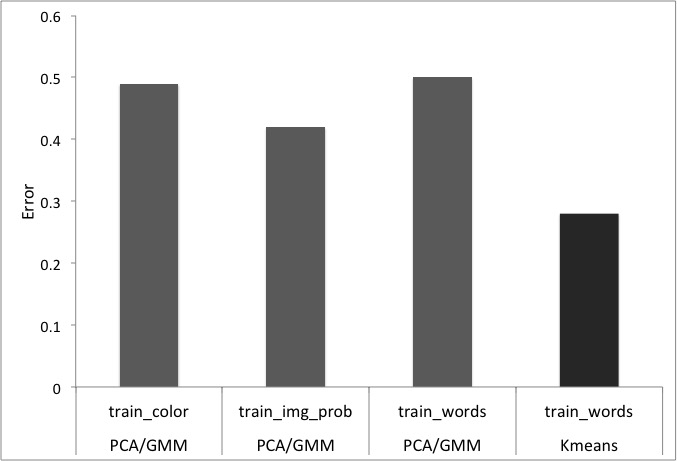
\includegraphics[scale=0.4]{trainingerror.jpg}
  \caption{Error of our Preliminary Methods}
  \label{fig:Error}
\end{figure}

\section{Main Methods}

Here we describe the combination of models we used in our final model. We used our Naive Bayes model to beat Baseline 1, 78\%, and our final to beat Baseline 2 and the final submission. 


\subsection{Naive Bayes}

For supervised learning, Naive Bayes classification is an effective generative method for classifying texts, such as identifying spam in email. The words\_train data uses bag of words model where counts of words matters and position of words does not matter. Although the conditional independence assumption of  Naive Bayes may not be true, the method is a dependable baseline for text classification and it trains fast. \\

We used the  Matlab function fitcnb on the words\_train dataset. To train the model, we used 10-fold cross validation and specified the bag-of-words model as the distribution parameter and the multinomial distribution. We chose these parameters because they had the lowest cross validation error of the other parameter specifications we tried.The model predicted very well, with a cross validation accuracy of 0.80 on the training, and 0.7962 on the test data (Figure 3). We successfully beat the Baseline 1 with this simple Naive Bayes model. \\

The dataset matrix for words is very sparse, and for each tweet there are thousands of words that do not appear. The Naive Bayes model for text classifications assumes that there is no information in words that are not observed and this may cause over-fitting. We can solve this by smoothing the Naive Bayes model, ensuring that each word gets a non-zero probability. The performance of the model drops when multiple features are correlated. We never checked the correlation between features, which could have been visualized with multiple sploms. 

\subsection{GentleBoost}

The second main method we utilized was an ensemble method. We used GentleBoost, a weak learning that was built by MATLAB under the fitensemble function. The method combines many weak learners into one high quality ensemble predictor. We chose this ensemble methods over the others offered by MATLAB, because it is preforms well with binary classification trees with many predictors. The input of the model was the word\_train data. We used a 10-fold cross validation method to observe how the model preformed, specified the use 300 learners, and the type of learner as 'tree'. The average cross validation error was 0.21 (Figure 3). The algorithm classified joy and sadness well. \\

The method could have improved if we increased the number of learners, however it would have taken a very long time to train because the data is large. Initially we tried the method with the default number of learners, 100 trees, and found that the cross validation accuracy only improved slightly. This slight improvement with triple number of learners reveals that the data has some intricacies or patterns that the ensemble method cannot learn.   


\subsection{Support Vector Machine}

Support vector machines (SVMs) proved to the most promising method to classify the data. We used the MATLAB function, fitcsvm, to train an SVM model for binary classification on the on the word\_train data.We tried a simple SVM by specifying a linear kernel, and had a  cross validation error was 0.2180. With a Gaussian or RBF kernel we had an error of 0.4373. After experimenting with a variety of kernels, we found that the linear preformed the best. fitsvm allows you to make an assumption about the fraction of outliers in the data. While we could have gone through the raw tweets and looked through the data, we decided to experiment with  10\%, 20\%, and 30\% and observed cross validation errors 0.2121, 0.2282, and 0.2131 respectively. Specifying the outliers percentage did not have an effect on our cross validation error, so we decided not to specify it in our SVM final model.  \\

Lastly we optimized our SVM by using MATLABs built in method to optimize a cross-validated SVM using Bayes Optimization.  The method originates from The Elements of Statistical Learning, Hastie, Tibshirani, and Friedman (2009). Paraphrasing from the MATLAB documentation,  the model begins with generating 10 base points 2 classes. For each of the classes, it generates 100 random points. After 100 points for each class has been generated, the point are classified using fitcsvm. The function bayesopt is used to optimize the parameters of the final SVM model with respect to cross validation." We submitted the method to the autograder, and it had an accuracy of 0.7991 (Figure 3). The method was accurate enough to beat Baseline 1, but not Baseline 2. \\

The selection of parameters is essential for obtaining the most accurate SVM. The model did not preform well because we did not find the best way to tune the parameters. The data was sparse and high dimensional, so the hyperplane would be able to separate the data well. Another method we should have tried is a logistic regression.

\section{Final Method}

Our final method utilizes sentiment analysis, the classification of text into categories of emotions. We used the vaderSentiment 2.4.1 package in Python. VADER is a lexicon and rule-based sentiment analysis tool that is specifically attuned to sentiments expressed in social media. The advantage of this analysis is that we can use this preliminary method to discern extremely positive and extremely negative tweets by assuming that there are no extremely positive words shown in negative sentences and vise versa. We will describe the process of experimenting with two analyzes before selecting one to include in our final model.

\subsection{Sentiment Analysis 1}

In Python, we ran a sentimental analysis on each word present in the topwords\.csv (Appendix). The input was each individual word in the list, and the output was the probability the word expresses a negative, positive, and neutral emotion. The output often looks like this, when type "funny" we can see \{'compound': 0.4404, 'neg': 0.0, 'neu': 0.0, 'pos': 1.0\}, which means it is an extremely positive word.

\subsection{Sentiment Analysis 2}

We did not consider the raw tweets containing words beginnings with \#. These hash tags may represent the topic this sentence belongs to, some specific topics always express similar emotions, like \#family usually expresses a positive emotion. So instead of analyzing the sentiment of each word, we used sentence as the input and received the average emotion scores of each word.We ran the sentimental analysis on each raw tweet. For all the words that appeared in this sentence, we attached the resulting score to those words. For every word, an average emotion score is then based on all the raw tweets.

\subsection{Final Method}

Our final method beat Baseline 2 and received an accuracy of 81.82\%. We trained the model 80\% of the training data and tested on the hold out data. The Sentiment Analysis predicted "sadness" with a 90\% accuracy. So the intuition was straight forward, if the hold out data calculated by Sentiment Analysis 1 had negative words and no positive words, we labeled it as negative. With the data the Sentiment Analysis would not predict, we had our Naive Bayes, SVM, and Gentle Boost models predict a label and decide the final label with a majority vote.Figure 2 details the structure of our final method. We have three models predicting the test labels, if three of them  predict a tweet as sadness, the label is sad, and similiarly for joy. If any two of them predict a tweet as sadness, we label it as sadness. Finally, if two of them predict a tweet as joy, we use the Naive Bayes label. Interestingly we observed that Naive Bayes have a higher training accuracy predicting joy than using majority vote method. We tried the same method with Sentimental Analysis 2, but the accuracy decreased (Figure 3). It may because the new Sentiment Analysis did not have that strong predictive words like Sentiment Analysis 1, or maybe the result of Sentiment Analysis 1 is more suitable to the test data.


\begin{figure}
	\centering
  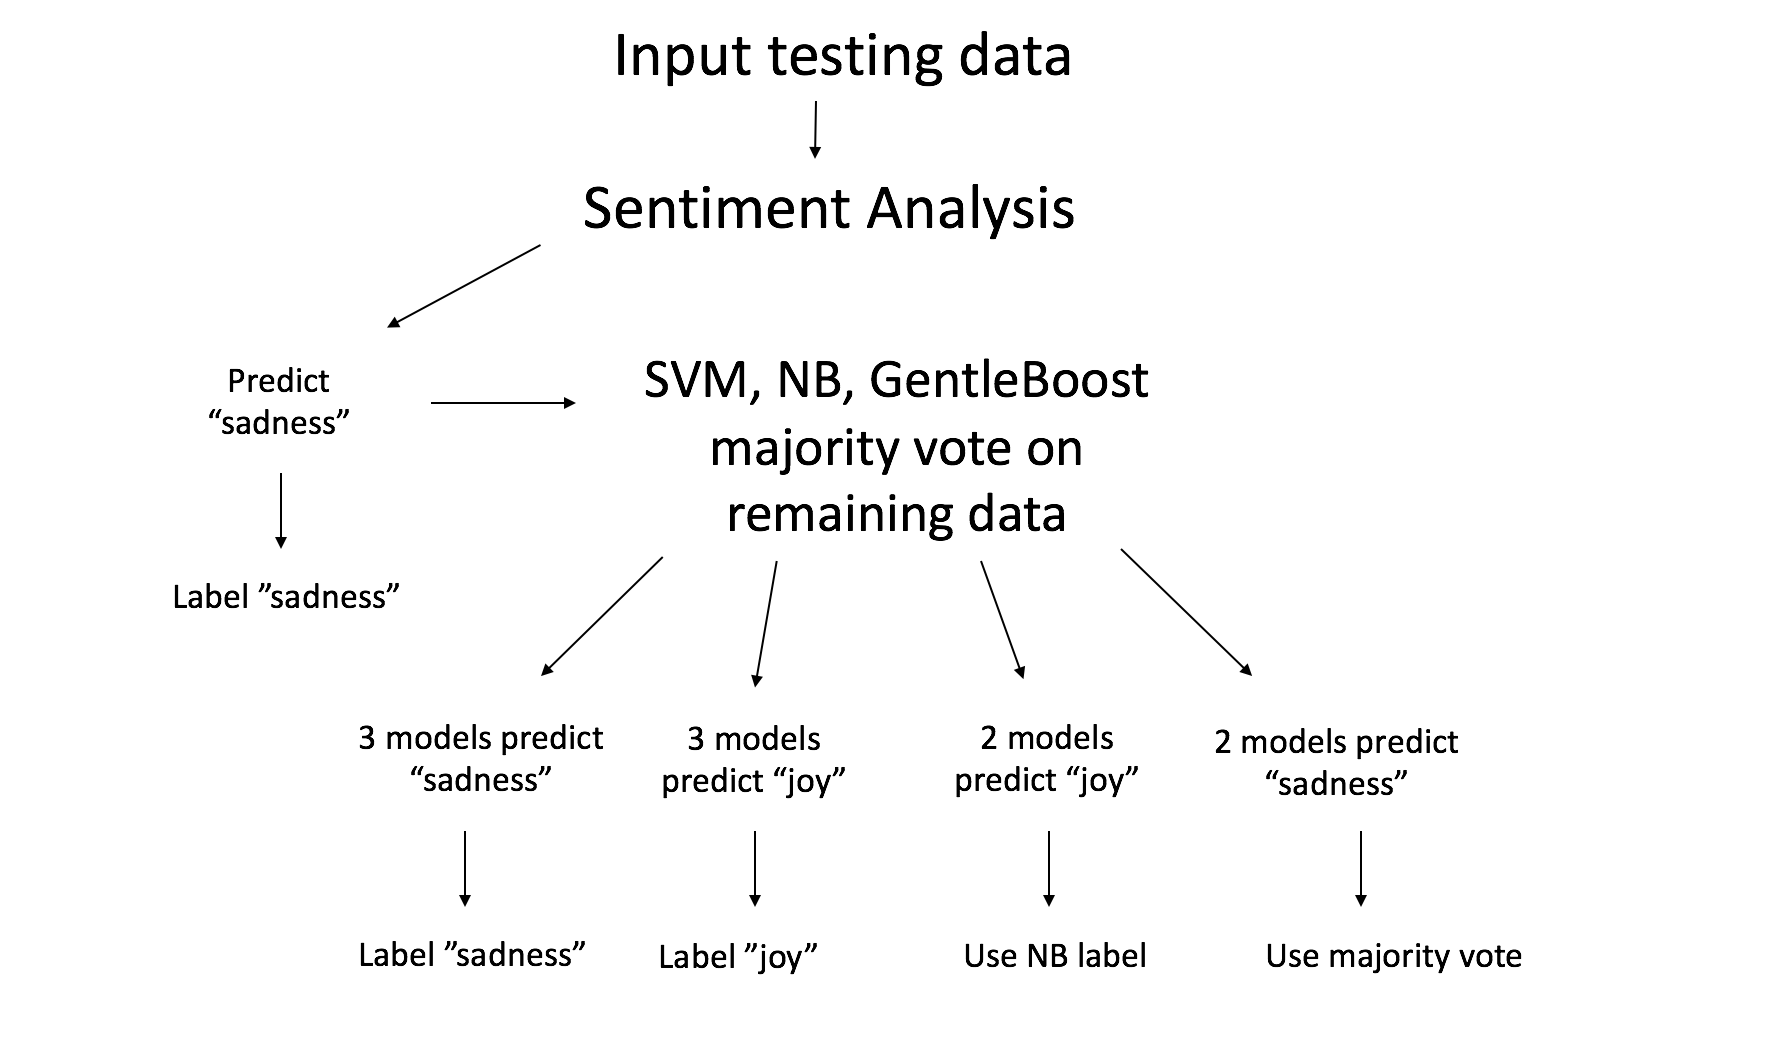
\includegraphics[scale=0.35]{Method.jpg}
  \caption{System Classification}
  \label{fig:System Classification}
\end{figure}

\begin{figure}
	\centering
  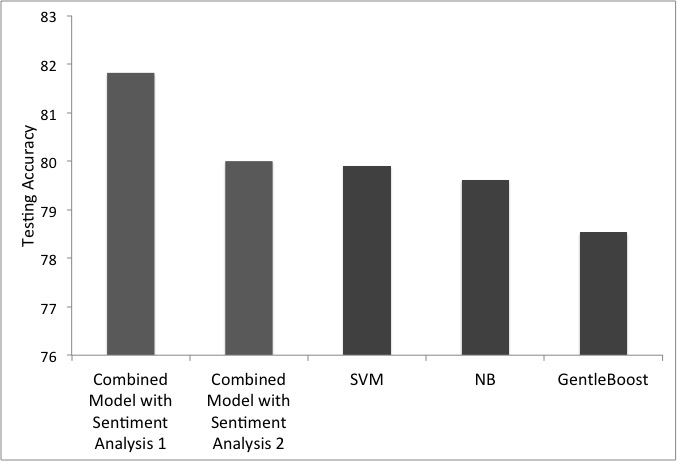
\includegraphics[scale=0.4]{FinalGraph.jpg}
  \caption{Test Error Final Models. The separate final models are in dark grey, and combined models with sentiment analysis are in light grey. The combined models have higher testing accuracy that the separate models. The combined model with sentiment analysis 2 preforms just as well as SVM. The model with Sentiment Analysis 1 has the highest testing accuracy.}
  \label{fig:Test Error}
\end{figure}

\section{Discussion}

Other methods we tried on words includes TF-IDF. TF-IDF is short for term frequency–inverse document frequency, and is a numerical statistic that is intended to reflect how important a word is to a document in a collection. We used this method to transform the words\_train data and then used SVM or logistic regression methods to predict labels. The errors were high, probably due to the fact that the the training data are too sprase, which is the nature of tweets.  \\

Classifying emotion is a difficult problem because human emotion is multifaceted and varies in intensity. In person, understanding the emotion a person is based on several parameters like the context of what they're saying, their words, tone, body language, and facial expression. Our classification problem is more difficult because we are given short tweets with a corresponding image. One idea to improve our method is by using a more update lexicon, assuming that the tweets are from 2015 or 2016. The lexicon used in the vaderSentiment 2.4.1 package is from 2014. In the last two years language in tweets has changed with the use of more emojis, hastags, 'fad' words such as 'bae', and the decrease in emoticons. An interesting method that we could have tried if we had time would be to train a classifer on emojis, emoticons, and hashtags. The three pieces generally represent the topic or feeling of a tweet. It would be interesting to test that hypothesis. 
\section{Appendix}

\lstinputlisting[language=Python]{"./sentimental analysis with python.py"}

\end{document}
